\chapter{評価手法と結果}
\label{chap:evaluation}
\section{本提案の評価概要}
本章では\ref{chap:implementation_and_experimentation}章で
述べたシミュレーションにおける結果についてまとめる.

\ref{section:要件1に対するシミュレーション結果}節では
\ref{section:要件定義}節で述べた配送遅延の増加抑制の効果について, 
\ref{section:2030年代の地球・月間のDTNを想定したシミュレーションのシナリオとパラメータ}節で述べた
地球-月間のシミュレーション, 
\ref{section:2040年代の地球・月・火星間のDTNを想定したシミュレーションのシナリオとパラメータ}節で述べた
地球-火星間の距離に応じた3種類のシミュレーションにおける
配送を試みたBundleの到達率とその平均遅延を示す. 

\ref{section:要件2に対する更新メッセージによるリンク消費}節では
\ref{section:要件定義}節で述べた運用面での効果について, 
上記それぞれのシミュレーションについて, 
運用上のデメリットとして既存手法における臨時更新メッセージが天体間のリンクを消費するか示す. 

\section{要件1に対するシミュレーションでの到達率・到達遅延の結果}
\label{section:要件1に対するシミュレーション結果}

\subsection{地球・月間のシミュレーション結果}
\label{section:地球・月間のシミュレーション結果}
\ref{section:2030年代の地球・月間のDTNを想定したシミュレーションのシナリオとパラメータ}節で述べた
地球-月間のシミュレーションについて, 配送を試みたBundleの到達率とその遅延は
それぞれ図\ref{fig:graph_bundle_earth_moon}と図\ref{fig:graph_delay_earth_moon}のようになった. 
実験の結果, 図\ref{fig:graph_bundle_earth_moon}に示す通り
臨時更新を行わない場合にはおよそ70\%のBundleは到達しなかった一方, 
既存手法と提案手法ではすべてのBundleが到達した.
また到達遅延に関しても, 図\ref{fig:graph_delay_earth_moon}に示す通り, 
既存手法とほぼ変わらない値となった. 
%地球・月間のシミュレーション結果
\begin{figure}[tbh]
    \centering
    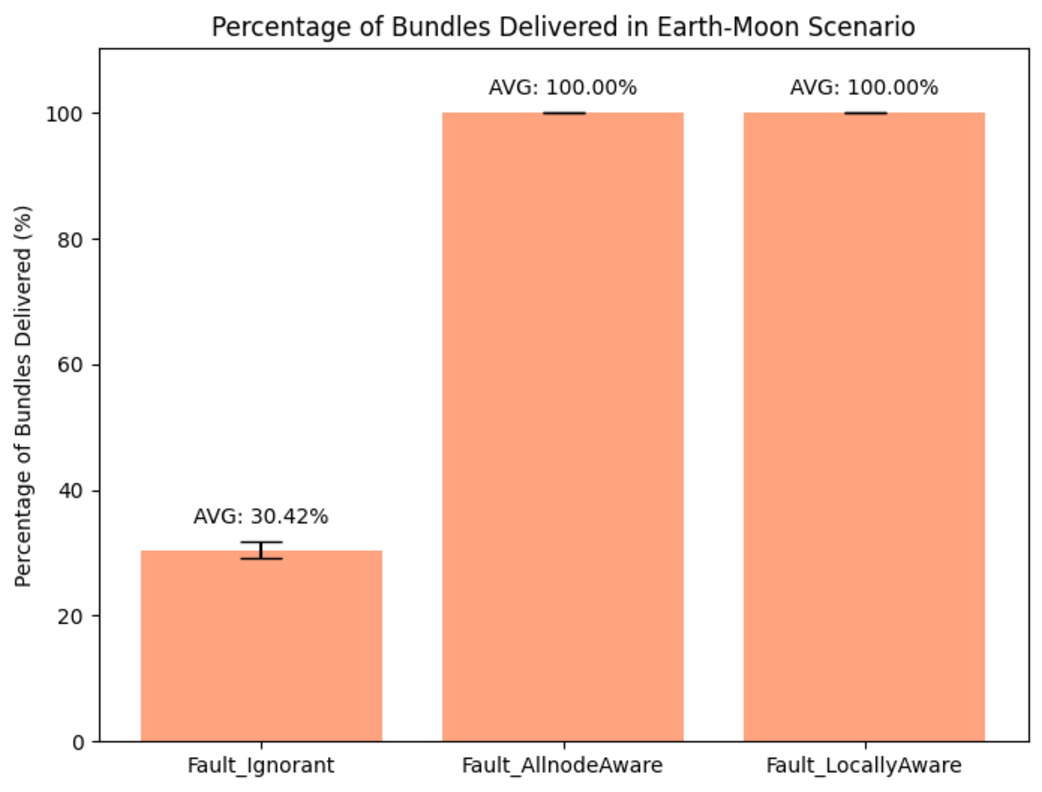
\includegraphics[width=0.7\textheight]{img/moon_bundle.pdf}
    \caption{地球・月間シナリオにおけるBundleの到達率}
    \label{fig:graph_bundle_earth_moon}
    \begin{minipage}{\textwidth}
        \centering
        \vspace{3mm}
        \fontsize{10.5pt}{12pt}\selectfont
        Contactの失敗情報について, どのノードにも拡散を行わない場合をFault\_Ignorant, 
        天体間を超えてすべてのノードに拡散する場合をFault\_AllnodeAware, 
        天体内のノードのみに拡散する場合をFault\_LocallyAwareとして表記した. 
    \end{minipage}
\end{figure}

\begin{figure}[tbh]
    \centering
    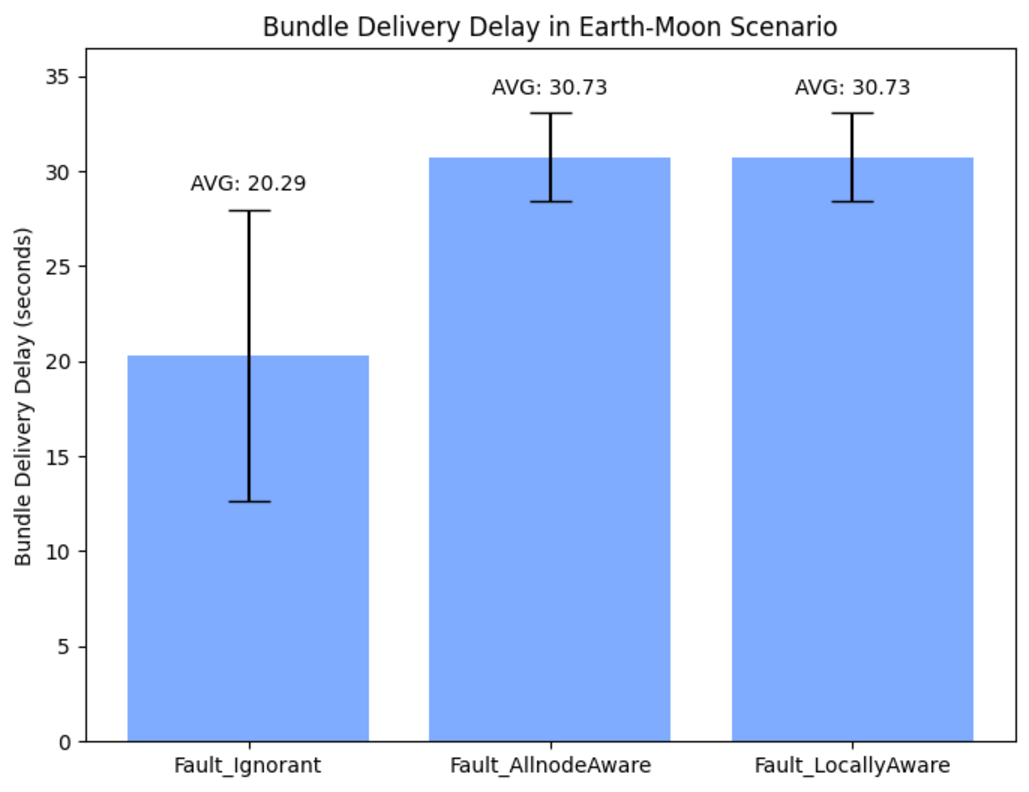
\includegraphics[width=0.7\textheight]{img/moon_delay.pdf}
    \caption{地球・月間シナリオにおけるBundleの到達遅延}
    \label{fig:graph_delay_earth_moon}
    \begin{minipage}{\textwidth}
        \centering
        \vspace{3mm}
        \fontsize{10.5pt}{12pt}\selectfont
        Fault\_Ignorant, Fault\_AllnodeAware, Fault\_LocallyAwareの表記は
        図\ref{fig:graph_bundle_earth_moon}と同様である.
    \end{minipage}
\end{figure}

\subsection{地球・月間のシミュレーション結果に対する考察}
\label{section:地球・月間のシミュレーション結果に対する考察}
提案手法では既存手法とほぼ同程度の遅延となり要件1に対する効果は非常に高かった. 
また臨時更新を行わない場合において到達遅延が低く計算されているのは, 
Contactの失敗に伴い到達できなかったBundleは到達遅延に含めないためである. 既存手法と提案手法ではこれらのBundleは
別なルートでルーティングされ, 平均到達遅延を大きく増加させるものの, 宛先ノードへの到達には成功している. 

\subsection{地球・火星間のシミュレーション結果}
\label{section:地球・火星間のシミュレーション結果}
\ref{section:2040年代の地球・月・火星間のDTNを想定したシミュレーションのシナリオとパラメータ}節で述べた
地球-火星間のシミュレーションについて, 配送を試みたBundleの到達率とその遅延は
地球-火星間の距離が480光秒の時について
図\ref{fig:graph_bundle_earth_mars_480}と図\ref{fig:graph_delay_earth_mars_480}のように, 
地球-火星間の距離が840光秒の時について
図\ref{fig:graph_bundle_earth_mars_840}と図\ref{fig:graph_delay_earth_mars_840}のように, 
地球-火星間の距離が1200光秒の時について
図\ref{fig:graph_bundle_earth_mars_1200}と図\ref{fig:graph_delay_earth_mars_1200}のようになった. 

地球-火星間の距離が480光秒と840光秒のシナリオにおいては, 
臨時更新を行わない場合には平均6\%程度しか到達しなかったが,
既存手法・提案手法で臨時更新を行なった場合には95\%を超える非常に多くのBundleが到達し, 
かつ提案手法と既存手法で到達率が完全に一致した.
また到達遅延に関しても, 提案手法と既存手法はともに遅延の値自体は大きかったものの, 両者の値は完全に一致した. 
\begin{figure}[tbh]
    \centering
    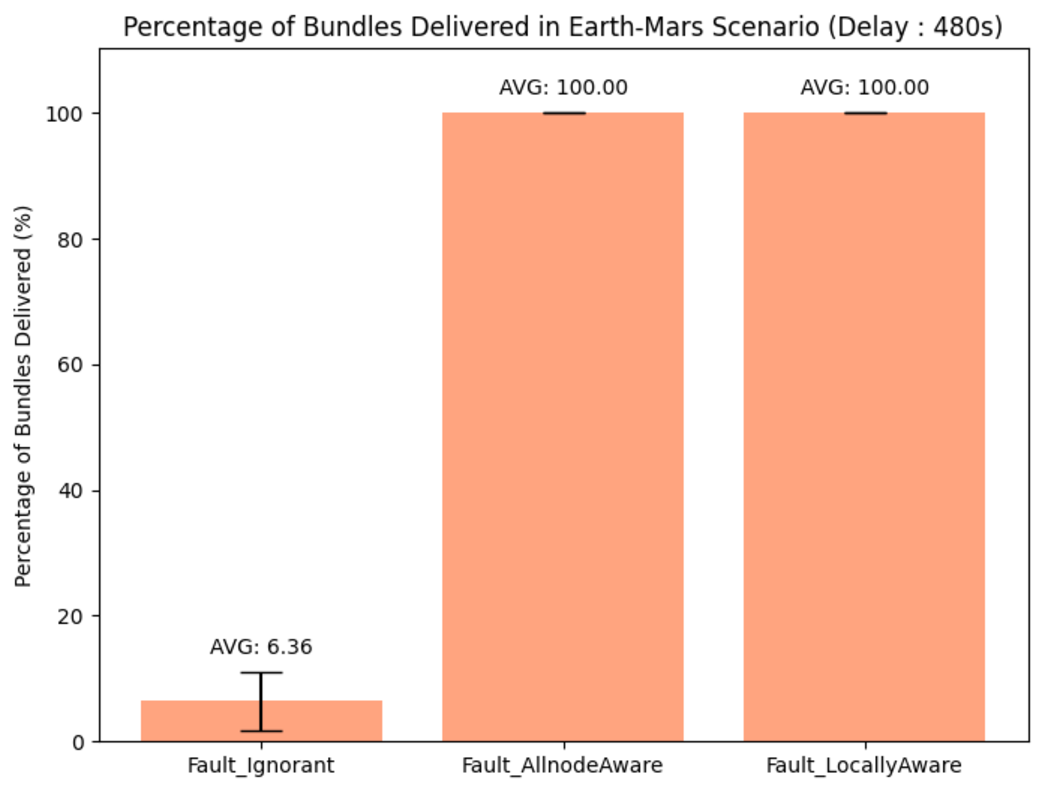
\includegraphics[width=0.7\textheight]{img/mars_480_bundle.pdf}
    \caption{地球・火星間シナリオ(距離480光秒)におけるBundleの到達率}
    \label{fig:graph_bundle_earth_mars_480}
    \begin{minipage}{\textwidth}
        \centering
        \vspace{3mm}
        \fontsize{10.5pt}{12pt}\selectfont
        Fault\_Ignorant, Fault\_AllnodeAware, Fault\_LocallyAwareの表記は
        図\ref{fig:graph_bundle_earth_moon}と同様である.
    \end{minipage}
\end{figure}

\begin{figure}[tbh]
    \centering
    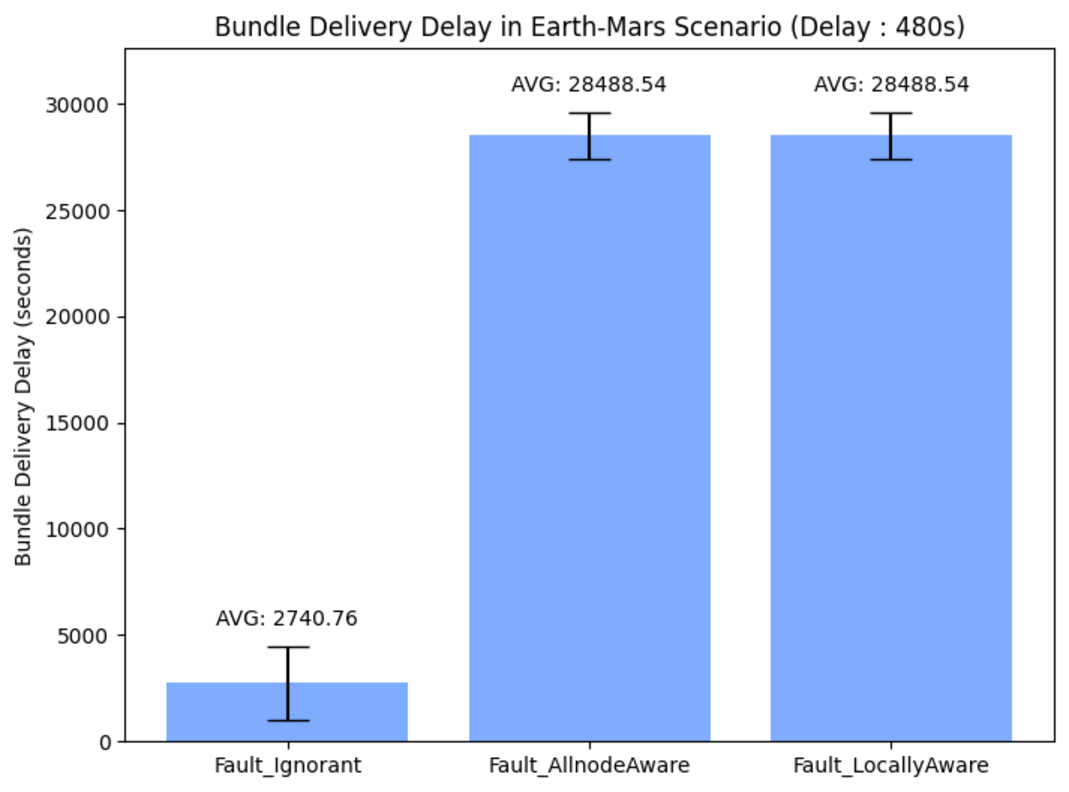
\includegraphics[width=0.7\textheight]{img/mars_480_delay.pdf}
    \caption{地球・火星間シナリオ(距離480光秒)におけるBundleの到達遅延}
    \label{fig:graph_delay_earth_mars_480}
    \begin{minipage}{\textwidth}
        \centering
        \vspace{3mm}
        \fontsize{10.5pt}{12pt}\selectfont
        Fault\_Ignorant, Fault\_AllnodeAware, Fault\_LocallyAwareの表記は
        図\ref{fig:graph_bundle_earth_moon}と同様である.
    \end{minipage}
\end{figure}

\begin{figure}[tbh]
    \centering
    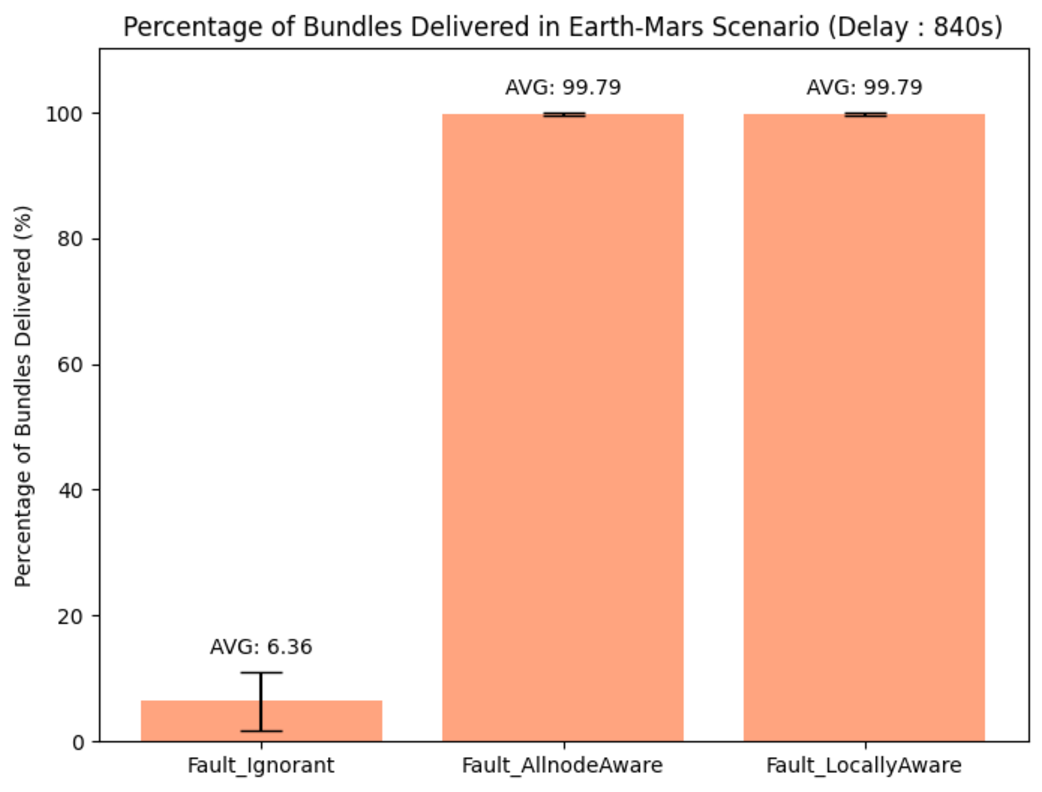
\includegraphics[width=0.7\textheight]{img/mars_840_bundle.pdf}
    \caption{地球・火星間シナリオ(距離840光秒)におけるBundleの到達率}
    \label{fig:graph_bundle_earth_mars_840}
    \begin{minipage}{\textwidth}
        \centering
        \vspace{3mm}
        \fontsize{10.5pt}{12pt}\selectfont
        Fault\_Ignorant, Fault\_AllnodeAware, Fault\_LocallyAwareの表記は
        図\ref{fig:graph_bundle_earth_moon}と同様である.
    \end{minipage}
\end{figure}

\begin{figure}[tbh]
    \centering
    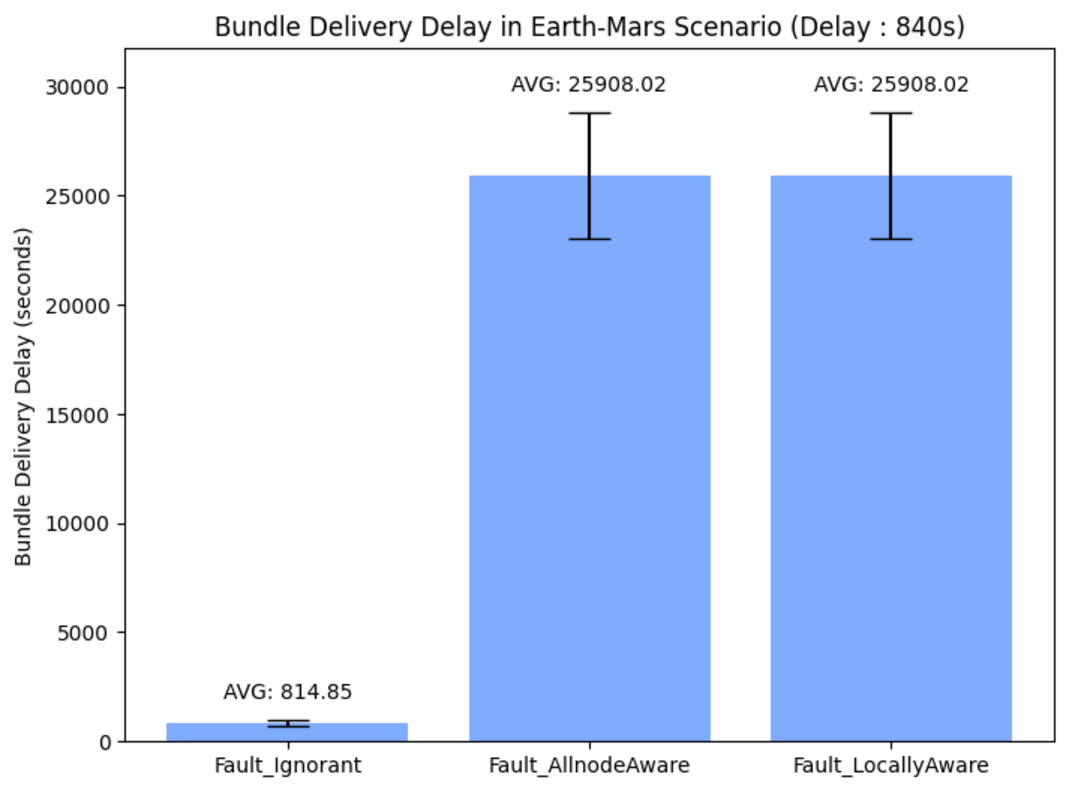
\includegraphics[width=0.7\textheight]{img/mars_840_delay.pdf}
    \caption{地球・火星間シナリオ(距離840光秒)におけるBundleの到達遅延}
    \label{fig:graph_delay_earth_mars_840}
    \begin{minipage}{\textwidth}
        \centering
        \vspace{3mm}
        \fontsize{10.5pt}{12pt}\selectfont
        Fault\_Ignorant, Fault\_AllnodeAware, Fault\_LocallyAwareの表記は
        図\ref{fig:graph_bundle_earth_moon}と同様である.
    \end{minipage}
\end{figure}

\begin{figure}[tbh]
    \centering
    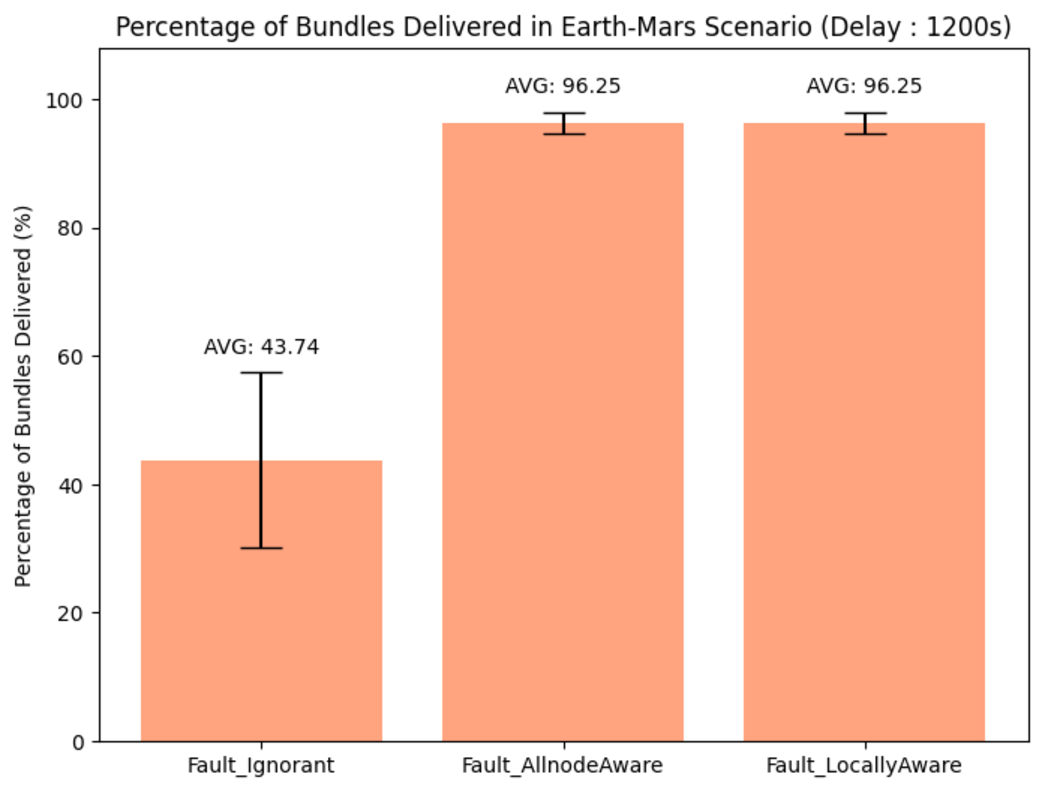
\includegraphics[width=0.7\textheight]{img/mars_1200_bundle.pdf}
    \caption{地球・火星間シナリオ(距離1200光秒)におけるBundleの到達率}
    \label{fig:graph_bundle_earth_mars_1200}
    \begin{minipage}{\textwidth}
        \centering
        \vspace{3mm}
        \fontsize{10.5pt}{12pt}\selectfont
        Fault\_Ignorant, Fault\_AllnodeAware, Fault\_LocallyAwareの表記は
        図\ref{fig:graph_bundle_earth_moon}と同様である.
    \end{minipage}
\end{figure}

\begin{figure}[tbh]
    \centering
    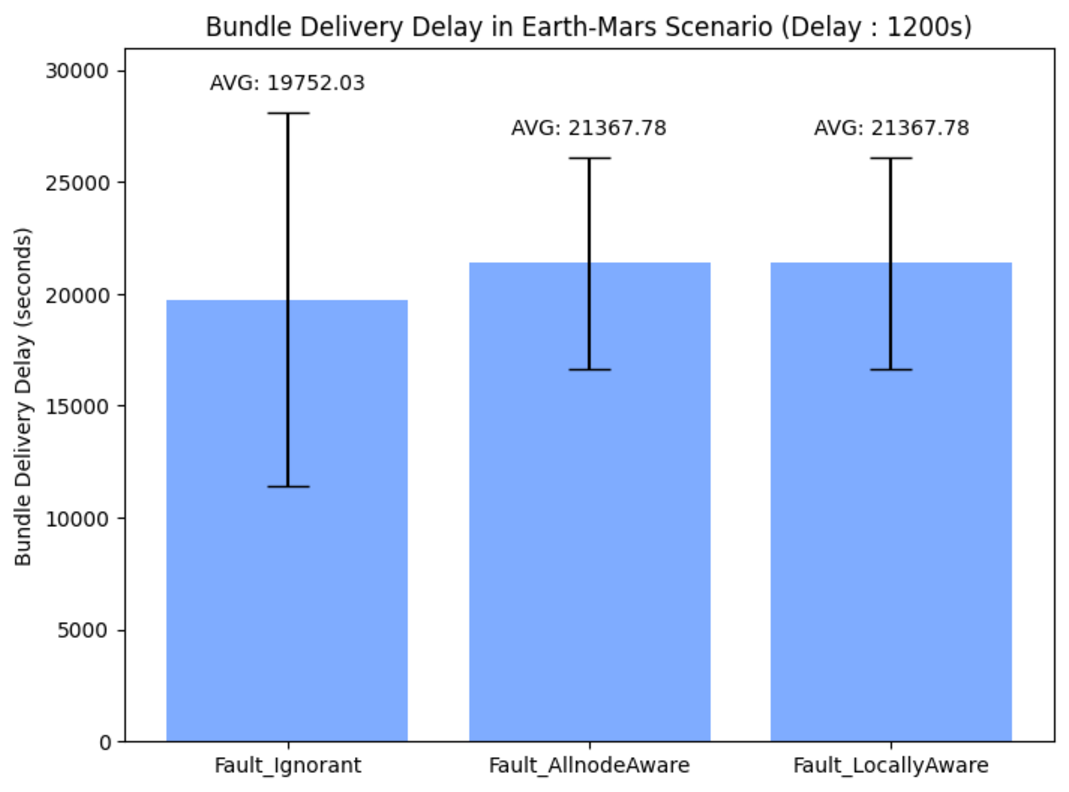
\includegraphics[width=0.7\textheight]{img/mars_1200_delay.pdf}
    \caption{地球・火星間シナリオ(距離1200光秒)におけるBundleの到達遅延}
    \label{fig:graph_delay_earth_mars_1200}
    \begin{minipage}{\textwidth}
        \centering
        \vspace{3mm}
        \fontsize{10.5pt}{12pt}\selectfont
        Fault\_Ignorant, Fault\_AllnodeAware, Fault\_LocallyAwareの表記は
        図\ref{fig:graph_bundle_earth_moon}と同様である.
    \end{minipage}
\end{figure}

\subsection{地球・火星間のシミュレーション結果に対する考察}
\label{section:地球・火星間のシミュレーション結果に対する考察}
図\ref{fig:graph_delay_earth_mars_480}, 
図\ref{fig:graph_delay_earth_mars_840}, 
図\ref{fig:graph_delay_earth_mars_1200}において
火星までのシミュレーションにおいて遅延が既存手法と提案手法で完全に一致している理由としては, 
地球-火星間の距離が遠いため, Contact失敗の発生後に選ばれる最適経路に, 
それ以前までの最適経路と比較して天体間の経路まで変更する経路が選ばれにくかったことが考えられる. 
図\ref{fig:example_of_routechange}における例で考えると, ノード4から6へのContactに失敗が生じ, 
経路1・R_{1 \rightarrow 2 \rightarrow 4 \rightarrow 6}に代わりに選ばれる最適な経路の候補として
経路2・R_{1 \rightarrow 2 \rightarrow 5 \rightarrow 6}もしくは
経路3・R_{1 \rightarrow 2 \rightarrow 4 \rightarrow 5 \rightarrow 6}が同時に存在する場合, 
(A) = D^{2}_{4}+D^{4}_{5} - D^{2}_{5}が正であれば経路2が, 負であれば経路3が最適経路として選ばれる. 
しかし(D^{2}_{4}とD^{2}_{5})は
地球-火星間が480光秒の時でD^{4}_{5}のおよそ3700倍程度, 
地球-火星間が840光秒の時でD^{4}_{5}のおよそ6500倍程度, 
地球-火星間が1200光秒の時でD^{4}_{5}のおよそ9200倍程度あり, 
またそれぞれのシミュレーションにおける, D^{2}_{4}とD^{2}_{5}の
そのシミュレーションにおける地球-火星間の距離の変動は1\%の範囲であるため, 
| D^{2}_{4} - D^{2}_{5} | >> | D^{4}_{5} | ・・・(B)となりやすい. 
さらにContactの失敗発生前には経路1が最適経路であった場合には, 
前提として経路1が経路2よりも優先されていた, すなわち(D^{2}_{4}+D^{4}_{6}-D^{2}_{5}-D^{5}_{6})が負であり, 
上記同様にD^{2}_{4} - D^{2}_{5} >> D^{4}_{6} - D^{5}_{6} を考慮するとD^{2}_{4} > D^{2}_{5} ・・・(C)となる. 
よって実際に(B)と(C)となっている場合, 

\begin{align}
    (A) &= D^{2}_{4} + D^{4}_{5} - D^{2}_{5} \notag \\
    &\fallingdotseq D^{2}_{4} - D^{2}_{5} (\because (B)) \\
    &> 0 \notag (\because (C)\notag)
\end{align}

となり, 経路2が選択される. 
これにより既存手法と提案手法において同様の経路が選択され到達率と到達遅延の結果が一致していると考えられる. 

\section{要件2に対する更新メッセージによるリンク消費と考察}
\label{section:要件2に対する更新メッセージによるリンク消費}
\ref{section:要件定義}節で述べたように, 既存手法では天体間での更新メッセージの送信が必要であり, 
その際にリンクを消費する. 一方, 本提案手法では自天体内のノードにのみ更新メッセージを送信するため, 
そのメッセージによる天体間リンクの消費は一切ない. 
本論文では図\ref{figure:cpup_pdu_format}および図\ref{figure:command_block_format}で示した
CPUPのPDUとその中のCommand Blockについては先行研究で用いられたフォーマットをそのまま用いることを想定する. 
1回のContact失敗とそれを知らせる更新のメッセージが単一のBundleで送信される場合, 
CPUPのPDUは以下のようになることが想定される. 

\begin{figure}[htbp]
    \centering
    \label{figure:delete_command_block_format}
    \begin{tabular}{|c|c|c|c|}
        \hline
        Byte 0 & Byte 1 & Byte 2 & Byte 3 \\
        \hline
        \multicolumn{1}{|c|}{Version num.} & \multicolumn{3}{c|}{Number of Command Blocks (SDNV)} \\
        \hline
        Byte 4 & Byte 5 & Byte 6 & Byte 7  \\
        \hline
        \multicolumn{2}{|c|}{Creation Timestamp (SDNV)} & \multicolumn{2}{c|}{Command Expiry (SDNV)} \\
        \hline
        Byte 8 & Byte 9 & Byte 10 & Byte 11 \\
        \hline
        \multicolumn{3}{|c|}{Command Originator (SDNV)} & Command Type \\
        \hline
        Byte 12 & Byte 13 & Byte 14 & Byte 15 \\
        \hline
        \multicolumn{4}{|c|}{ID of Contact to delete} \\
        \hline
    \end{tabular}
    \caption{既存手法における単一のContactを削除するCPUPのCommand Block}
  \end{figure}

リンク消費量は以下のようになった. 
\begin{equation}
    \text{リンク消費量} = \text{CPUPのPDUのサイズ} \times \text{削除するContact数}
\end{equation}

\ref{section:2030年代の地球・月間のDTNを想定したシミュレーションのシナリオとパラメータ}節で述べた地球-月間のシナリオにおいては, 
生成した600回のContactのうち200回のContactを失敗させるシナリオであるため, リンク消費量は以下のようになる. 
\begin{equation}
    \text{リンク消費量} = 16 \text{Bytes} \times 200 \text{個のContact削除メッセージ} = 3200 {Bytes} 
\end{equation}

\ref{section:2040年代の地球・月・火星間のDTNを想定したシミュレーションのシナリオとパラメータ}節で述べた地球-火星間のシナリオにおいては, 
生成した480回のContactのうち100回のContactを失敗させるシナリオであるため, リンク消費量は以下のようになる. 
\begin{equation}
    \text{リンク消費量} = 16 \text{Bytes} \times 100 \text{個のContact削除メッセージ} = 1600 {Bytes} 
\end{equation}
